\documentclass[dvipdfmx,a4paper]{standalone}
\usepackage{tikz}
\usetikzlibrary{arrows,positioning}
\begin{document}
	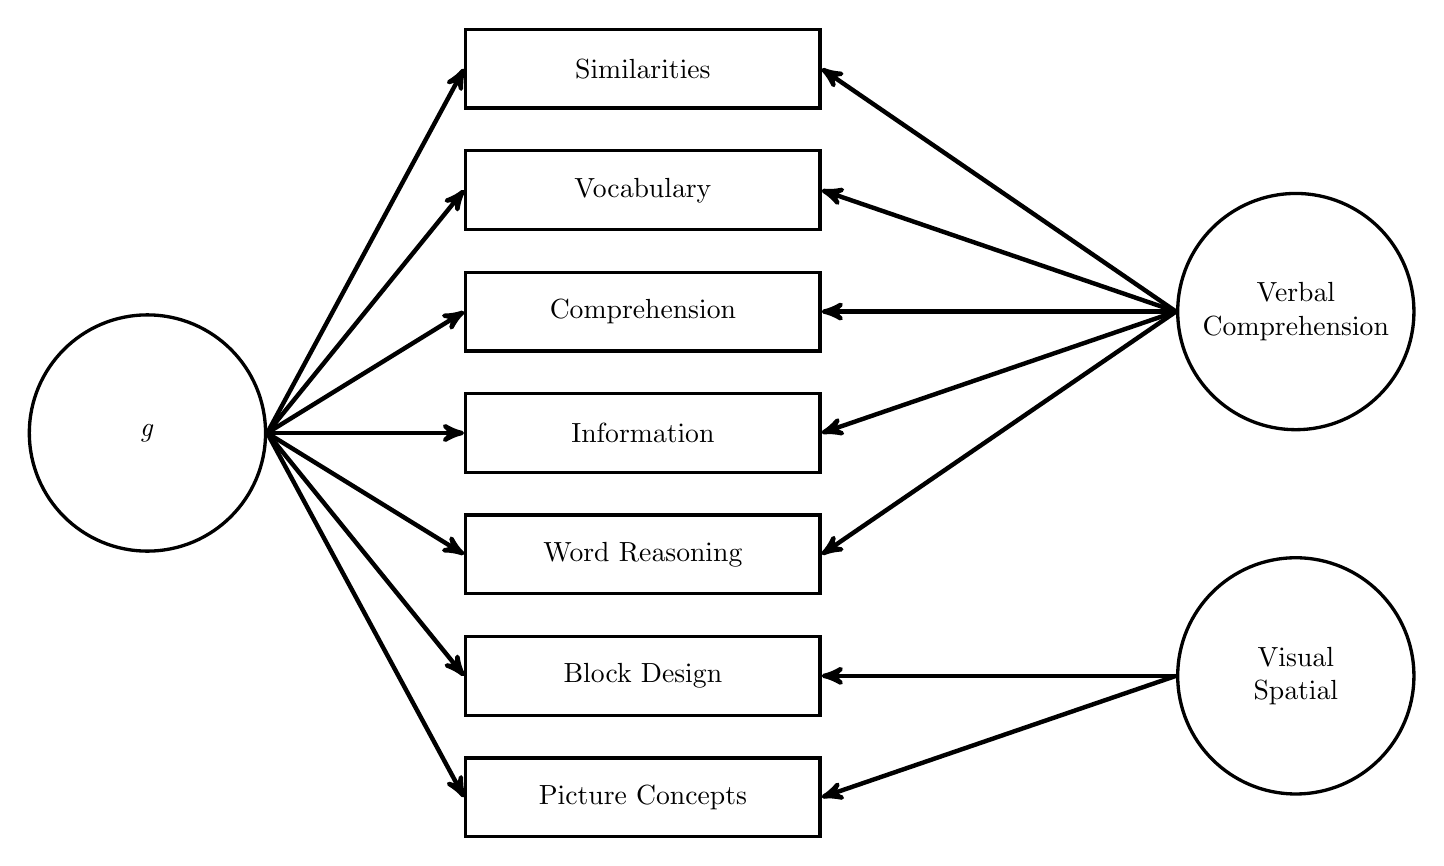
\begin{tikzpicture}[auto,node distance=.5cm,
	latent/.style	={circle,draw,very thick,inner sep=0pt,minimum size=30mm,align=center},
	manifest/.style	={rectangle,draw,very thick,inner sep=0pt,minimum width=45mm,minimum height=10mm},
	paths/.style	={->, ultra thick, >=stealth'},
	]
	
	\node [manifest] (SI) at (0,0) {Similarities};
	\node [manifest] (VO) [below=of SI] {Vocabulary};
	\node [manifest] (CO) [below=of VO] {Comprehension};
	\node [manifest] (IN) [below=of CO] {Information};
	\node [manifest] (WR) [below=of IN] {Word Reasoning};
	\node [manifest] (BD) [below=of WR] {Block Design};
	\node [manifest] (PS) [below=of BD] {Picture Concepts};
	\node [latent] (g) [left=2.5cm of IN] {\emph{g}};
	\node [latent] (Gc) [right=4.5cm of CO] {Verbal\\ Comprehension};
	\node [latent] (Gv) [right=4.5cm of BD] {Visual\\ Spatial};
	
	\foreach \all in {SI, VO, CO, IN, WR, BD, PS}
	{
		\draw [paths] (g.east) to node { } (\all.west);
	}
	
	\foreach \vc in {SI, VO, CO, IN, WR}
	\draw [paths] (Gc.west) to node {} (\vc.east);
	
	\foreach \vs in {BD, PS}
	\draw [paths] (Gv.west) to node {} (\vs.east);
	\end{tikzpicture}
\end{document}